%\documentclass[a4paper]{article}
\usepackage[utf8]{inputenc}
\usepackage[spanish, es-tabla, es-noshorthands]{babel}
\usepackage[table,xcdraw]{xcolor}
\usepackage[a4paper, footnotesep = 1cm, width=22cm, top=2.5cm, height=25cm, textwidth=20cm, textheight=25cm]{geometry}
%\geometry{showframe}

\usepackage{tikz}
\usepackage{amsmath}
\usepackage{amsfonts}
\usepackage{amssymb}
\usepackage{float}
\usepackage{graphicx}
\usepackage{caption}
\usepackage{subcaption}
\usepackage{multicol}
\usepackage{multirow}
\usepackage{wrapfig}
\setlength{\doublerulesep}{\arrayrulewidth}
\usepackage{booktabs}

\usepackage{hyperref}
\hypersetup{
    colorlinks=true,
    linkcolor=blue,
    filecolor=magenta,      
    urlcolor=blue,
    citecolor=blue,    
}

\newcommand{\note}[1]{
	\begin{center}
		\huge{ \textcolor{red}{#1} }
	\end{center}
}

\setcounter{topnumber}{2}
\setcounter{bottomnumber}{2}
\setcounter{totalnumber}{4}
\renewcommand{\topfraction}{0.85}
\renewcommand{\bottomfraction}{0.85}
\renewcommand{\textfraction}{0.15}
\renewcommand{\floatpagefraction}{0.8}
\renewcommand{\textfraction}{0.1}
\setlength{\floatsep}{5pt plus 2pt minus 2pt}
\setlength{\textfloatsep}{5pt plus 2pt minus 2pt}
\setlength{\intextsep}{5pt plus 2pt minus 2pt}

\newcommand{\quotes}[1]{``#1''}
\usepackage{array}
\newcolumntype{C}[1]{>{\centering\let\newline\\\arraybackslash\hspace{0pt}}m{#1}}
\usepackage[american]{circuitikz}
\usetikzlibrary{calc}
\usepackage{fancyhdr}
\usepackage{units} 

\graphicspath{{../Ejercicio-1/}{../Ejercicio-2/}{../Ejercicio-3/}{../Ejercicio-4/}{../ParteI/}{../ParteII/}{../ParteIII/}{../ParteIV/}}

\pagestyle{fancy}
\fancyhf{}
\lhead{22.14 - Electrónica IV}
\rhead{Mechoulam, Lambertucci, Londero}
\rfoot{Página \thepage}

%
%\begin{document}

\subsection{Diseño del sistema}

En el sistema que se busca desarrollar, se emplean los siguientes valores para la fuente Flyback:
\begin{multicols}{2}
\begin{itemize}
	\item $D = 0.3$
	\item $L_1 = 40 \ \mu H$
	\item $R_1 = R_3 = 10 \ \Omega$
	\item $C_1 = C_3 = 47 \ \mu F$
	\item $C_2 = C_4 = 2 \ \mu F$
	\item $\frac{N_1}{N_2} = 3 $
	\item $N_2 = N_3 $
\end{itemize}
\end{multicols}

Para el circuito del SG3525 se adoptaron los siguientes valores
\begin{multicols}{2}
\begin{itemize}
	\item $R_T = 2.2  \ k\Omega$
	\item $C_T = 3.3 \ n F$
	\item $R_D = 0 \ \Omega$
	\item $C_{ss} = 1 \ \mu F$
\end{itemize}
\end{multicols}

calculando el ripple a la salida se obtiene

\begin{equation}
0.05 = \frac{\Delta V_o}{V_o} = \frac{DT_s}{R_oC}
\end{equation}

\begin{equation}
C = \frac{DT_sV_o}{R_oC\Delta V_o} = 8.8 \mu F

\end{equation}

por lo que se seleccionó una combinación de capacitores con una capacitancia total de $\approx$ 48$\mu F$ siendo el paralelo de 1 capacitor electrolítico,3 cerámicos (2 de 1$\mu$F y uno de 68pF). Esta combinación se realiza con la intención de no solo aumentar la capacidad de salida, sino que tambien reducir la ESR neta de salida.  


La combinación de valores de $R_T$ y $C_T$ fueron elegidas para mantener la frecuencia de switching elegida. La resistencia $R_D$ es nula para que se descargue lo mas rápido posible. Por último, el capacitor $C_{ss}$ es para que tenga un comienzo suave.
Para la salida se utilizarón los diodos MUR160 y para el snubber se utilizó el diodo Schottky.  
\begin{figure}[H]
	\centering
	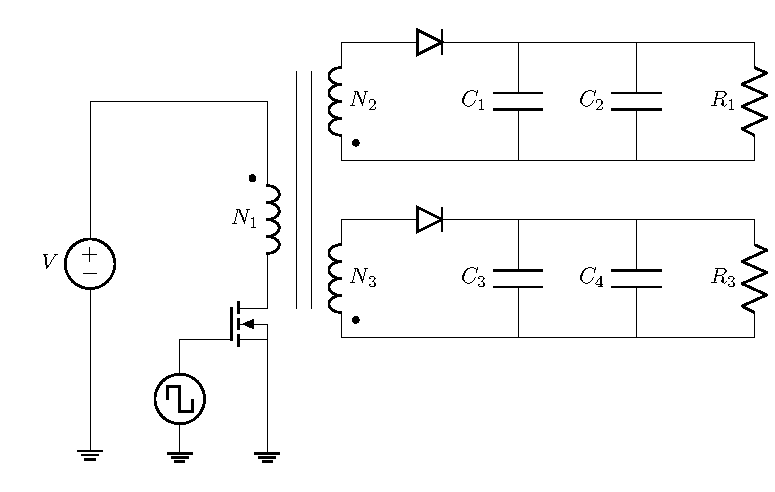
\includegraphics[width=0.7\linewidth, page = 1]{ImagenesParteII/Flyback.pdf}
	\label{fig:fly}
	\caption{Circuito del snubber empleado.}
\end{figure}

\subsection{Simulaciones}

\note{EXPLICAR OBSERVACIONES}
Se simuló el circuito a lazo abierto. De esta forma se obtuvieron las siguientes curvas.
\begin{figure}[H]
	\centering
	\includegraphics[width=0.9\linewidth]{ImagenesParteII/vos.png}
	\label{fig:vos}
	\caption{Variaciones en la $V_{out}$ al cambiar la $V_{comp}$.}
\end{figure}

Para la tensión que provoca la máxima corriente de salida se obtuvieron los siguientes gráficos:
\begin{figure}[H]
	\centering
	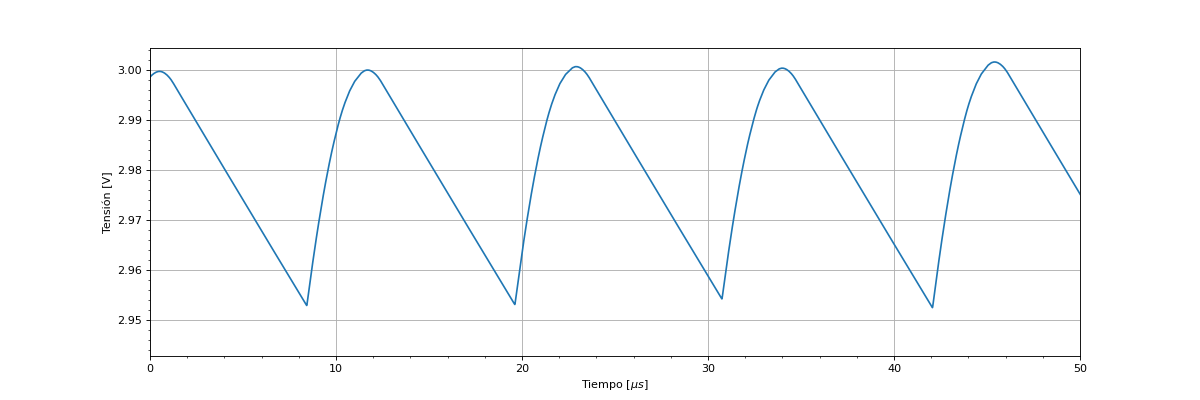
\includegraphics[width=\linewidth]{ImagenesParteII/ Vo.png}
	\label{fig:vo}
	\caption{Tensión de salida.}
\end{figure}

\begin{figure}[H]
	\centering
	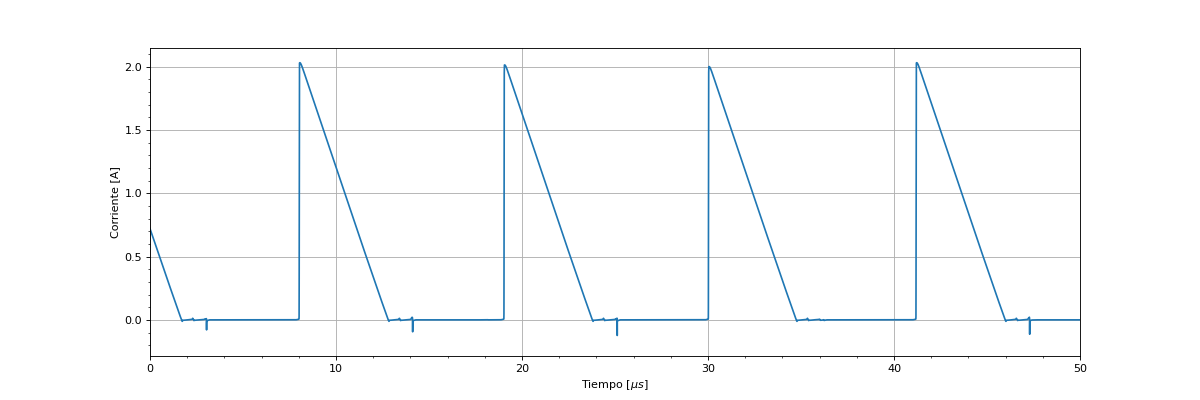
\includegraphics[width=\linewidth]{ImagenesParteII/Idiodo.png}
	\label{fig:idiodo}
	\caption{Corriente del diodo.}
\end{figure}

\begin{figure}[H]
	\centering
	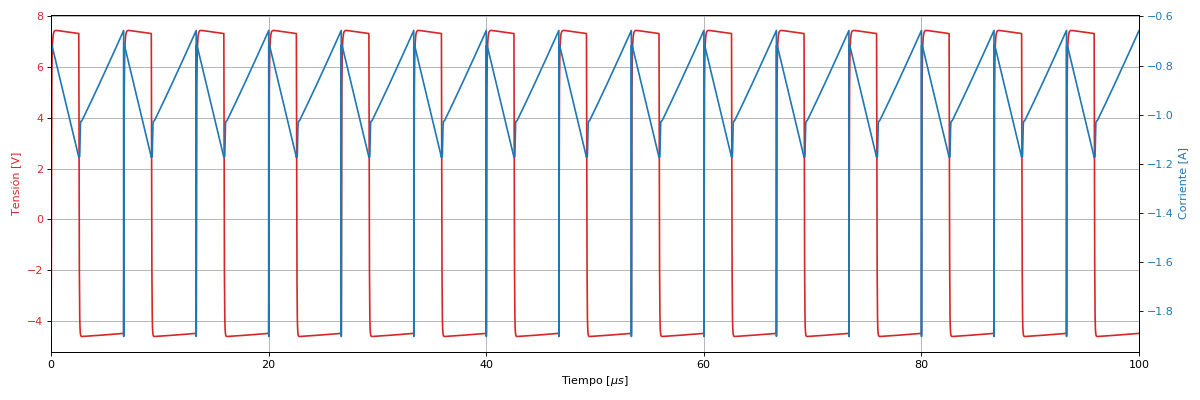
\includegraphics[width=0.9\linewidth]{ImagenesParteII/Primario.png}
	\label{fig:primario}
	\caption{Tensión y corriente del primario.}
\end{figure}

\begin{figure}[H]
	\centering
	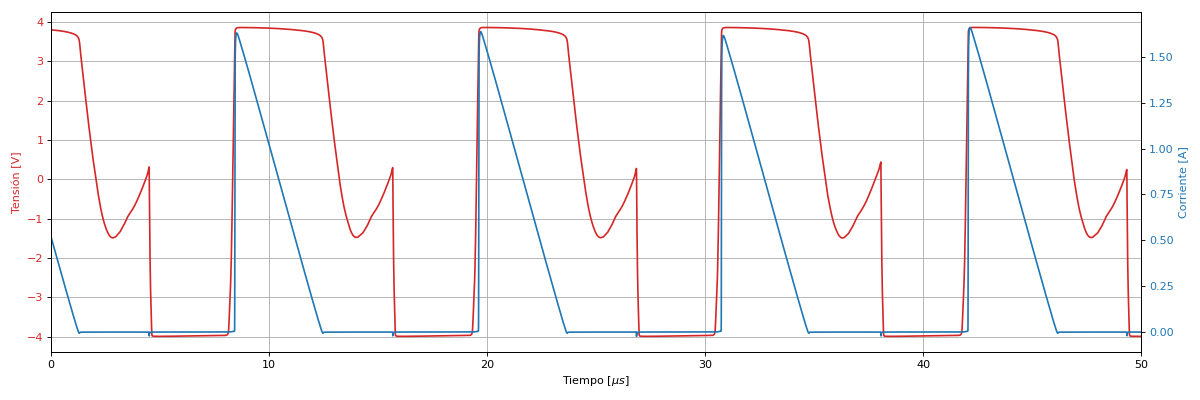
\includegraphics[width=0.9\linewidth]{ImagenesParteII/Secundario.png}
	\label{fig:secundario}
	\caption{Tensión y corriente del secundario.}
\end{figure}

\begin{figure}[H]
	\centering
	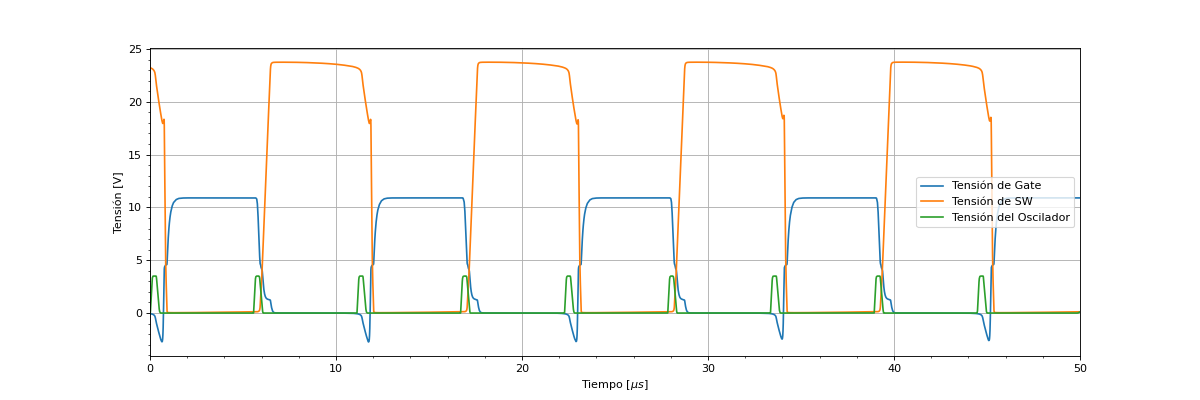
\includegraphics[width=\linewidth]{ImagenesParteII/TensionesVarias1.png}
	\label{fig:tensionesvarias}
	\caption{Tensión de Gate y del Switch.}
\end{figure}

\subsection{Snubber}
Para el circuito dado, se diseña un snubber empleando un diodo, una resistencia y un capacitor.
\begin{figure}[H]
	\centering
	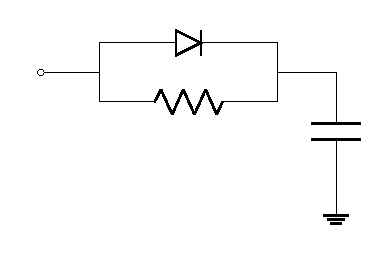
\includegraphics[width=0.3\linewidth, page = 1]{ImagenesParteII/Snubber.pdf}
	\label{fig:snubber}
	\caption{Circuito del snubber empleado.}
\end{figure}

Se calcula el valor máximo del capacitor, planteando que la energía entregada por la inductancia de dispersión debe ser absorbida completamente por el capacitor del snubber. De esta forma, se llega a la expresión:
%\begin{equation}
%	C > L_d \left( \frac{I_{L1}}{V_{C}} \right)^2 = 1 \ \mu H \cdot \left( \frac{15 \ A}{100 \ V} \right)^2 = 33 \ nF
%\end{equation}
\begin{equation}
	C > L_d  \frac{{I_{L1}}^2}{{V_{C}}^2 - \left( V_{CC} - V_{o} \frac{N_1}{N_2} \right)^2 } = 1 \ \mu H \cdot \frac{15 \ A}{{100 \ V}^2 - \left( 12 \ V - 3 \cdot 0.8 \ V \right)^2} = 23 \ nF
\end{equation}

De esta forma, se selecciona $C = 35 \ nF$. Planteando que tres veces el tiempo característico del sistema RC debe ser menor al tiempo en que el transistor se encuentra encendido, para así descargar completamente al capacitor, se obtiene una restricción similar para la resistencia. Operando, se llega a:
%\begin{equation}
%	R < \left. \frac{DT_S}{3C} \right|_{C = 10 \ nF} = \frac{0.5}{150 \ kHz} \cdot \frac{1}{3 \cdot 10 \ nF} = 111.11 \ \Omega
%\end{equation}
\begin{equation}
	R < \left. \frac{DT_S}{3C} \right|_{C = 10 \ nF} = \frac{0.5}{100 \ kHz} \cdot \frac{1}{3 \cdot 35 \ nF} = 71 \ \Omega
\end{equation}

Finalmente se selecciona $R = 47 \ \Omega$.

\begin{figure}[H]
	\centering
	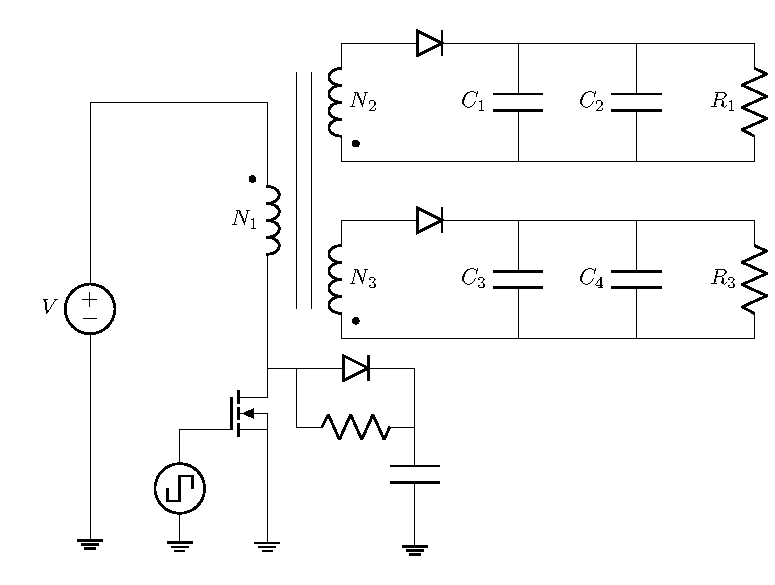
\includegraphics[width=0.4\linewidth, page = 1]{ImagenesParteII/FlybackSnubber.pdf}
	\label{fig:fly_snubber}
	\caption{Circuito Flyback con snubber.}
\end{figure}
Para el diodod el snubber se optó por el diodo 
\begin{figure}[H]
	\centering
	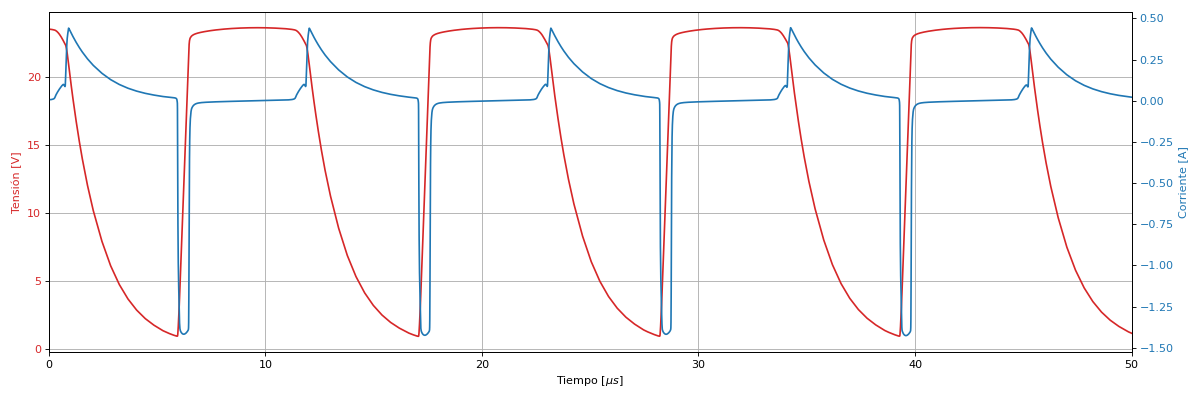
\includegraphics[width=0.9\linewidth]{ImagenesParteII/Cap_snub.png}
	\label{fig:tensionesvarias}
	\caption{Tensión y corriente en el capacitor de snubber.}
\end{figure}

\subsection{Potencias}
Las potencias teóricas calculadas son:
\begin{itemize}
\item $ P_{MOS} =\frac{f_{sw}}{2}\cdot V_{sw}I_{N1-min} t_{sw2}\ =\frac{88 \ kHz}{2}\cdot (21 \ V) \cdot (400 \ mA) \cdot (300 \ ns) = 110\ mW$
\item $ P_{RSnubber} = \frac{C{V_C}^2 F_{sw}}{2}\ = 679 \ mW$
\item $P_{diodo} = (I_o{R_d}^2 + I_oV_D)DT_sF_{sw} + P_{Irr} = saludos$ 

\end{itemize}
Las medidas en la simulación son:
\begin{itemize}
\item $ P_{MOS} = 45 \ mW $
\item $ P_{RSnubber} = 388.6 \ mW$
\item $ P_{diodo} = 258.35 \ mW$
\end{itemize}

\subsection{Eficiencia}
Se calculó la eficiencia del circuito de la siguiente manera:
%\note{PONER EN FUNCION DE LA CARGA Y DESDE LAMINIMA POTENCIA A LA SALIDA A LAMAXIMA}
\begin{equation}
\eta =\frac{P_{Load}}{P_{d}} = \frac{2 \cdot V_o^2 / R_L}{2 \cdot V_o^2 / R_L + \frac{CV_C^2 F_{sw}}{2} + \frac{f_{sw}}{2} \cdot V_{sw} \left( \frac{V_o / R_L}{1-D} \cdot \frac{N_2}{N_1} - \frac{V_o}{2L_2 \cdot f_{sw}} \cdot (1-D) \frac{N_1}{N_2}  \right) t_{sw2} } \Big\rvert_{V_o=3 V\ \& \ R_L=6.25 \Omega } = 70.35\%
\end{equation}
Para el gráfico se tomó una resistencia mínima de 0.71 $\Omega$ dado que con este valor satura el transformador y una máxima de 50$\Omega$.
\begin{figure}[H]
	\centering
	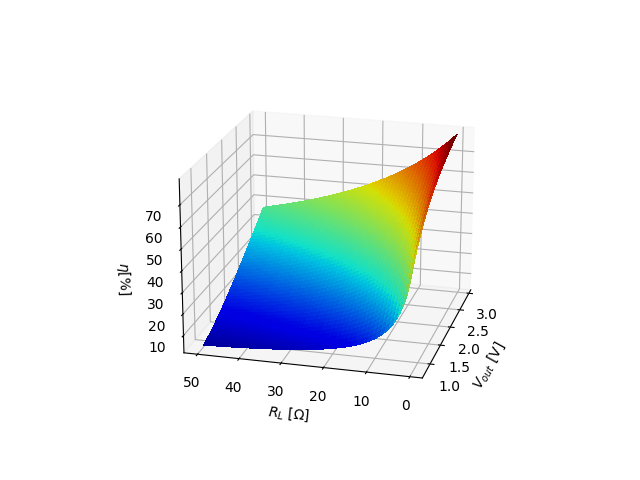
\includegraphics[width=0.5\linewidth]{ImagenesParteII/Eff.png}
	\label{fig:etar}
	\caption{Eficiencia en función de la carga y tensión.}
\end{figure}
Se observa que la combinación que da la mayor eficiencia tiende 
mientras que la simulada corresponde a baja carga y alta tensión.\\
Luego se obtuvo la eficiencia en la simulación.
\begin{equation}
\eta = 87\%
\end{equation}
%\end{document}
